\scrollmode                    % To exit upon error
\documentclass[letterpaper,twoside,12pt]{article}
\usepackage{polyglossia}
\setmainlanguage{russian}
%\setmainfont{Times New Roman} % Change to another font if Times New Roman fails
\newfontfamily\cyrillicfont{Times New Roman} % Specify the Cyrillic font

\usepackage[margin=0.8in]{geometry}
\usepackage{amsmath}
\usepackage{unicode-math} % For Unicode math support
\usepackage{graphicx}

%\title{\text{Расчёт выделения тепла в бухте-удлинителе}}
\title{Расчёт выделения тепла в бухте-удлинителе}

\author{Бенкевич Л. В.}

\begin{document}

\maketitle 

\emph{Задача.} Нагреватель воды \emph{паспортной} мощностью $P^*_\text{Н} = 2200 \, \text{Вт}$ подсоединён к сети напряжением $U = 220 \, \text{В}$ через удлинитель, длинный двужильный кабель длиной $l = 50 \, \text{м}$ и сечением каждой из двух жил $a = 0.75 \, \text{мм}^2$. Кабель-удлинитель смотан в бухту (размеры и число витков не имеют значения, пусть будет диаметр ~ 20-30 см). \\

Найти тепловую мощность, выделяемую в бухте кабеля.


\begin{figure}[h]
    \centering
    \begin{minipage}{0.45\textwidth}
        \centering
        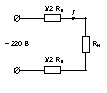
\includegraphics[width=\linewidth]{circuit_Rb_Rn_Rb.pdf}
        \caption{Сопротивления одной жилы кабеля, $\frac{1}{2} R_\text{Б}$, нагрузки (нагревателя воды), $R_\text{Н}$, и другой жилы кабеля, $\frac{1}{2} R_\text{Б}$,  в бухте.}
        \label{rb_rn_rb}
    \end{minipage}
    \hfill
    \begin{minipage}{0.45\textwidth}
        \centering
        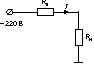
\includegraphics[width=\linewidth]{circuit_Rb_Rn.pdf}
        \caption{Сопротивления обеих жил кабеля в бухте, $R_\text{Б}$, и нагрузки (нагревателя воды), $R_\text{Н}$.}
        \label{rb_rn}
    \end{minipage}
\end{figure}


\emph{Решение.} Заметим, что ток последовательно протекает через три сопротивления (Рис.~\ref{rb_rn_rb}): жилу кабеля, $\frac{1}{2} R_\text{Б}$, сопротивление нагревателя воды, $R_\text{Н}$, и возвращается через другую жилу кабеля, $\frac{1}{2} R_\text{Б}$. Поскольку последовательные сопротивления складываются, мы можем эту схему упростить, заменив эквивалентной, состоящей из полного сопротивления бухты, $R_\text{Б}$, и нагревателя, $R_\text{Н}$ (Рис.~\ref{rb_rn}).

Сначала найдём все сопротивления, затем ток через них, а потом – мощность $P_\text{Б}$, выделяемую этим током в бухте.

Сопротивление провода определяется удельным сопротивлением меди, 
$\rho = 0.0172 \frac{\text{Ом мм}^2}{\text{м}}$, его сечением $a$ и длиной $l$: 
\begin{equation}
  \label{r_rhola}
  R = \rho\frac{l}{a}.
\end{equation}
Полное сопротивление кабеля в бухте, то есть последовательное сопротивление обеих жил $R_\text{Б}$, требует умножения длины кабеля на 2: 
\begin{equation}
  \label{r_buh}
  R_\text{Б} = \rho\frac{2l}{a} = (0.0172 \frac{\text{Ом\,мм}^2}{\text{м}}) \times (2 \cdot 50 \text{м}) / 
                                 (0.75 \text{мм}^2) = 2.293 \,\text{Ом}.
\end{equation}
Найдём сопротивление нагревателя $R_\text{Н}$ по его паспортной мощности $P^*_\text{Н}$, то есть той его мощности, которую нагреватель развивает, когда к его клеммам приложено ровно 220 В. При напряжении $U$ на концах сопротивления $R$ в нём выделяется тепловая мощность $P$ в соответствии с формулой
\begin{equation}
  \label{r_u2r}
  P = \frac{U^2}{R}; \quad \text{тогда} \quad R = \frac{U^2}{P}.
\end{equation}
Подставим наши числа:
\begin{equation}
  \label{r_nagr}
  R_\text{Н} = \frac{(220 \, \text{В})^2}{2200 \, \text{Вт}} = 22 \, \text{Ом}.
\end{equation}
По закону Ома, ток $I$ через наши два сопротивления будет
\begin{equation}
  \label{ohms_law}
  I = \frac{U}{R_\text{Б} + R_\text{Н}} = \frac{220~\text{В}}{2.293~\text{Ом} + 22~\text{Ом}} = (220/24.293)~A =
                                                                                                 9.056~A.
\end{equation}

Хоть это в задаче и не спрашивается, но ради интереса можно найти теперь \emph{реальное} напряжение на нагревателе,
\begin{equation}
  \label{г_nagr}
  U_\text{Н} = R_\text{Н} I = (22~\text{Ом}) \times (9.056~A) = 199.234~\text{В}.
\end{equation}
и его \emph{реальную} выделяемую тепловую мощность:
\begin{equation}
  \label{p_nagr}
  P_\text{Н} = I^2 R_\text{Н} = (9.056~A)^2 \times (22~\text{Ом}) = (82.013 \cdot 22)~\text{Вт} = 1804.287~\text{Вт}.
\end{equation}

Точно так же (хоть это и не спрашивалось в задаче) находим сумму напряжений, падающих на одну и другую жилы кабеля в бухте,
\begin{equation}
  \label{u_buh}
  U_\text{Б} = R_\text{Б} I = (2.293~\text{Ом}) \times (9.056~A) = 20.766~\text{В}.
\end{equation}

И, наконец, вычисляем тепловую мощность, выделяемую  в бухте сетевого удлинителя:
\begin{equation}
  \label{p_buh}
  P_\text{Б} = I^2 R_\text{Б} = (9.056~A)^2 \times (2.293~\text{Ом}) = (82.013 \cdot 22)~\text{Вт} = 188.055~\text{Вт}. 
\end{equation}

Таким образом, длинный и компактно смотанный сетевой кабель выделяет почти 200 Вт в своём небольшом объёме, что и приводит к его перегреву.

Можно добавить, что на этом длинном кабеле падает десятая часть напряжения, почти 21 В из 220 В, и до нагревателя доходит лишь 199 В вместо 220 В "паспортных".

\end{document}






%\begin{figure}[ht!]
%%  \begin{center}
%  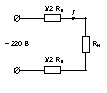
\includegraphics[width=20pc]{circuit_Rb_Rn_Rb.pdf}
%  \caption{\small \text{Сопротивления одной жилы кабеля, нагрузки (нагревателя воды) и другой жилы кабеля в бухте.}}
%  \label{rb_rn_rb}
%%  \end{center}
%\end{figure}


%\begin{figure}[ht!]
%  \begin{center}
%  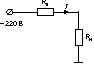
\includegraphics[width=20pc]{circuit_Rb_Rn.pdf}
%  \caption{\small \text{Сопротивления обеих жил кабеля в бухте и нагрузки (нагревателя воды).}}
%  \label{rb_rn}
%  \end{center}
%\end{figure}


